\documentclass[a4paper,10pt]{article}
% - a4paper: printing paper format
% - 10pt: size of the characters

\usepackage{graphicx}
\usepackage{titling}
\usepackage{listings}
\usepackage[table]{xcolor}
\newcolumntype{R}[1]{>{\raggedleft\arraybackslash }b{#1}}
\newcolumntype{L}[1]{>{\raggedright\arraybackslash }b{#1}}
\newcolumntype{C}[1]{>{\centering\arraybackslash }b{#1}}
\lstset{%
  basicstyle=\scriptsize\sffamily,%
  commentstyle=\footnotesize\ttfamily,%
  frameround=trBL,
  frame=single,
  breaklines=true,
  showstringspaces=false,
  numbers=left,
  numberstyle=\tiny,
  numbersep=10pt,
  keywordstyle=\bf
}
\newcommand{\subtitle}[1]{%
  \posttitle{%
    \par\end{center}
    \begin{center}\large#1\end{center}
    \vskip0.5em}%
}



%%%%%%%%%%%%%%%%%%%%%%%%%%%%%%%%%%%%%%%%%%%%%%%%%%%%
%				Title / Subtitle / Authors and Date									   %
% This should be adapted to your report.					                                                              %
%																			   %
%%%%%%%%%%%%%%%%%%%%%%%%%%%%%%%%%%%%%%%%%%%%%%%%%%%%
\title{TD3 : Formatted I/O Library}
\subtitle{Master M1 MOSIG, Grenoble Universities}
\author{Lenka Kun\'{i}kov\'{a} \and Lina Marsso}
\date{26/10/2014}

\begin{document}
% Beginning serious stuff. 


\maketitle
% Actually prints title / subtitle / authors and dat into the document


%%%%%%%%%%%%%%%%%%%%%%%%%%%%%%%%%%%%%%%%%%%%%%%%%%%%
%								Abstract										   %
% Change the part below the abstract so that it corresponds to your report	                                     %
%																			   %
%%%%%%%%%%%%%%%%%%%%%%%%%%%%%%%%%%%%%%%%%%%%%%%%%%%%

%%%%%%%%%%%%%%%%%%%%%%%%%%%%%%%%%%%%%%%%%%%%%%%%%%%%
%								Introductio	n									   %
%																			   %
% the command \section{name of the section} begins a new section of the document                            %
%																			   %
%%%%%%%%%%%%%%%%%%%%%%%%%%%%%%%%%%%%%%%%%%%%%%%%%%%%
\section{Introduction}
	\paragraph{}
	In this project we have to implement a I/O  library. 
	And evaluate their performances in different applications.
	\paragraph{}
	Firstly in this report we give answers of questions in the subject. 
	Then we present you our implementation.
	Then we speak about the safety checks implementation. 
	Finnaly, we analyse the performance and conclude this project.

\section{Subject questions}
\subsection{Question 1}


\section{Implementation}	
\subsection{Struct my\_file}
 Our structure my\_file consists of buffer in which we temporarily store information that we read from a file or that user tried to write in. We use two pointers that show us in which part of the buffer are valid data. Of course, we need to remember handler we got from the system call write / read. We also have variables to distinguish between read and write mode, to remember if we already met EOF and one that knows whether buffer was already filled or it is empty.  
 \subsection{my\_fopen}
 In this function we allocate the memory needed for the whole structure and we initialise all variables. Both pointers will point to the beginning of the buffer. According to the specified mode we open the file with appropriate flags.
 \subsection{my\_fclose}
 In this function we need to close the file and free all allocated memory. If the mode of file is set to write, we also need to write the content of the buffer into the file.

 \subsection{my\_fread}
 At first, the function should check whether the mode is set to read, if not, it returns -1. Then we need to distinguish between different cases. In case it is the first read operation, the buffer is empty and we need to fill it. In case the amount of data the user requests to read is less than data available, it is the simplest case and we just give requested data to the user. Another case is when we meet EOF before expected. It can be detected thanks to the pointer that points to the end of valid data. In this case we just give user less data than he wanted. It can also happen that user wants more than what is disponsible in the buffer. In this case, we give him all we have, we refill the buffer and give him remaining data. We keep refilling data until we get enough.

 \subsection{my\_fwrite}
 As in the previous function, we should test whether the mode is set to write. If it is, user data will be stored. If there is enough space in the buffer, we just write all user data in. Once the buffer is full, we write its content in a file using actual system call. We keep writing data in and flushing full buffer until all user data are processed.

\section{Safety checks}

\section{Evaluation}
\paragraph{}
For evaluate our library, we use one test he copie one file in an
other file buffered for our library and we write the same test 
but using the standard open, read and write.
\paragraph{}
We evaluate in the begining the time for copy two file with our library, 
and with the standard open, read and write. We have also one ratio~: 
\begin{equation}
\left(\frac{My\_stdio\_time\_execution}{Standar\_Read\_Write\_time\_execution} \right)  \quad
\end{equation}
\paragraph{}
We calculate the time of the execution with a script time.sh. We can see
for example in table 5.1, the ratio is 4/36. Our library is also 9 time
more fast. 

\subsection{Table with time execution of two differents test}
\begin{tabular}{|R{2cm}|C{2cm}|L{1.5cm}|L{1.5cm}|}
\hline \rowcolor{lightgray}Library & Time (microsecondes) & Size of file\\
\hline  libmy\_sdio & 4 & 8.0K \\
\hline  Standar  & 36 & 8.0K \\
\hline 
\end{tabular}

\begin{figure}[ht]
\center 
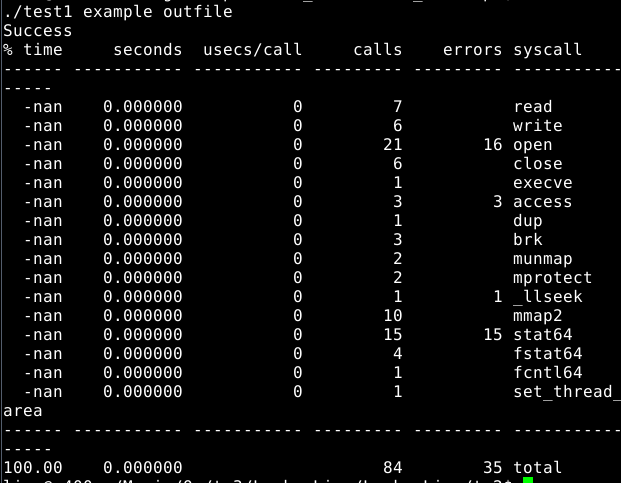
\includegraphics[width=0.85\linewidth]{my_strace.png}
\caption{Number of system call of our library}
\label{first}
\end{figure}
\begin{figure}[ht]
\center 
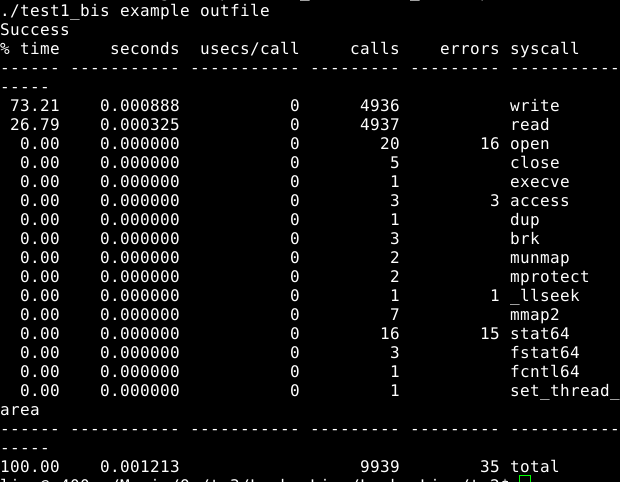
\includegraphics[width=0.85\linewidth]{syscall_strace.png}
\caption{Number of system call with read and write}
\label{worst}
\end{figure}
\begin{figure}[ht]
\center 
%\includegraphics[width=0.8\linewidth]{gcc_best_fit.png}
\caption{Memory requested and memory used with best fit strategy}
\label{best}
\end{figure}

\subsection{Table with fragmentation level of differents programs}

\begin{tabular}{|R{2cm}|C{1.5cm}|L{1.5cm}|L{1.5cm}|}
\hline \rowcolor{lightgray}program & worst\_fit & best\_fit & first\_fit \\
\hline  ls & 1.83 & 1.83 & 2.48 \\
\hline  wc & 0.96 & 0.96 & 0.96 \\
\hline  ps & 1.37 & 1.36 & 1.37 \\
\hline  hostname & 2.42 & 2.42 & 3.23 \\
\hline 
\end{tabular}

\section{Conclusion}
\paragraph{}
The goal of this project was to get familiar with the concept of memory 
managment and I think we succeeded. We managed to implement a simple 
version of memory allocator which allows users to allocate and free memory.
\paragraph{} 
During the implementation we had to deal with several problems. For 
example we needed to find a way on how to determine positions of free 
blocks when we do not have linked lists of them, or think about the 
algorithm that helps us merge contiguous blocks of free space. Moreover, 
we implemented the three most common algorithms for finding an appropriate 
free block (first-fit, best-fit and worse-fit). We are now able to describe 
pros and cons for each of them.
\paragraph{}
In the second part, we added some other features to our memory allocator. 
All of them related to security checks. Now we know that implementing 
functions for free and alloc memory is not enough and we also need 
to deal with situations where users (on purpose or by chance) do not act the 
way we expect. The control we are making is not perfect but it helps 
us to deal with many cases that may happen.

\paragraph{}
Finnaly, we can see an application of our allocator. We can analyse it's
performance with many apllications like ls, hostname... It was a very 
interesting project.

 \end{document}
